\chapter{Introducción}
\label{chap:introduccion}

\drop{S}{olamente} en 2018, el \textbf{Museo Reina Sofía} de Madrid recibió 3,9 millones de vistantes, aproximadamente un 2\% más que el año anterior. Del mismo modo, el \textbf{Museo de Prado} recibió casi 3 millones, un 2,4\% más que en 2017. Otro ejemplo de esto es el Macba, el Museo de Arte Contemporáneo de Barcelona, que recibió en 2018 casi 332,000 visitantes, un 28\% más que el año anterior\footnote{\url{https://www.abc.es/cultura/arte/abci-museos-espanoles-crecen-2018-201901021635_noticia.html}}. Con estos datos, puede verse que el interés por los museos está creciendo.

Pero la industrias de ocio que indiscutible más dinero genera es la \textbf{industria de videojuegos}, que solo en 2018 generó 43 mil millones de dólares, un 18\% más que en 2017\footnote{\url{https://tcrn.ch/2HtFczS}}. Por dar un contexto de estas cifras, en 2016 la suma conjunta del cine y la música solo generó 815 millones de dólares\footnote{\url{https://www.elperiodico.com/es/ocio-y-cultura/20180827/videojuegos-cine-musica-cultura-comparativa-7001883}}.

Por ello, en han comenzado a nacer nuevas maneras de jugar y nuevas técnicas de interacción con los usuarios, como la \textbf{Realidad Virtual}. La Realidad Virtual es un paradigma que intenta presentar a los jugadores con experiencias lo más \textbf{inmersivas} posible, para lo que hace uso de la visión estereoscópica de las personas.

Además, los dispositivos que permiten hacer uso de estas tecnologías se están abaratando mucho, hasta el punto de que un jugador casual puede permitirse un headset \acs{VR} para jugar ocasionalmente. 

\section{Motivación}

Siempre he estado muy interesado en el desarrollo de videojuegos; cuando era pequeño, y siempre que podía, intentaba jugar a cualquier videojuego que pudiera, y según crecía me empecé a interesar más y más por el proceso técnico que había detrás, así que empecé a ver documentales de desarrollo de videojuegos hasta que empecé a desarrollarlos yo.

Durante el grado, que estudié en la Universidad de Castilla-La Mancha, tuve la suerte de coincidir con algunos profesores que también estaban muy interesados en este tema y que habían organizado dos cursos; el primero, en 2015, fue el \textbf{Curso de Desarrollo de videojuegos multi-plataforma para dispositivos móviles}\footnote{\url{http://www.curso-openfl.cedv.quijost.com/}}, un curso de 100 horas en el que desarrollamos un pequeño juego en 2D en Haxe utilizando el framework OpenFL.

Tras él, dos años más tarde hice el \textbf{Curso de Experto en desarrollo de videojuegos}\footnote{\url{http://cedv.es}}, de 750 horas, en el que realizamos varios proyectos en C++ utilizando el motor de gráficos Ogre3D y otras tecnologías como CEGUI o Bullet.

A raíz de estos cursos, y por el uso que el dimos, comencé a interesarme más por Blender, un programa de diseño 3D que integra todos los componentes necesarios para modelar, texturizar, animar y renderizar toda clase de proyectos.

Y en este contexto nace \textit{MineRVa}. Por un lado, nunca había trabajando con entornos de desarrollo específicos para videojuegos, como Unity o Unreal Engine, y ni mucho menos con tecnologías de Realidad Virtual, lo que me pareció un reto importante y me llamó la atención desde el principio.

Por otro, aunque ya que aunque había trabajado desarrollando sistemas interactivos nunca lo había hecho aplicando metodologías adecuadas, por lo que este proyecto parecía el contexto perfecto para aprender.

\section{Entorno}

El entorno de ejecución de \MineRVa está compuesto por unas gafas de Realidad Virtual, dos controladores y un ordenador personal. Por tanto, el programa final debe ser lo suficientemente ligero en cuanto a recursos para poder ser ejecutado en un ordenador no especialmente potente.

La figura \ref{fig:entorno} presenta un ejemplo de ejecución en el que se puede ver al usuario de \MineRVa llevando el headset \acs{VR} y los mandos mientras juega en una de las escenarios iniciales.

\vspace{0.4cm}

\begin{figure}[!h]
\begin{center}
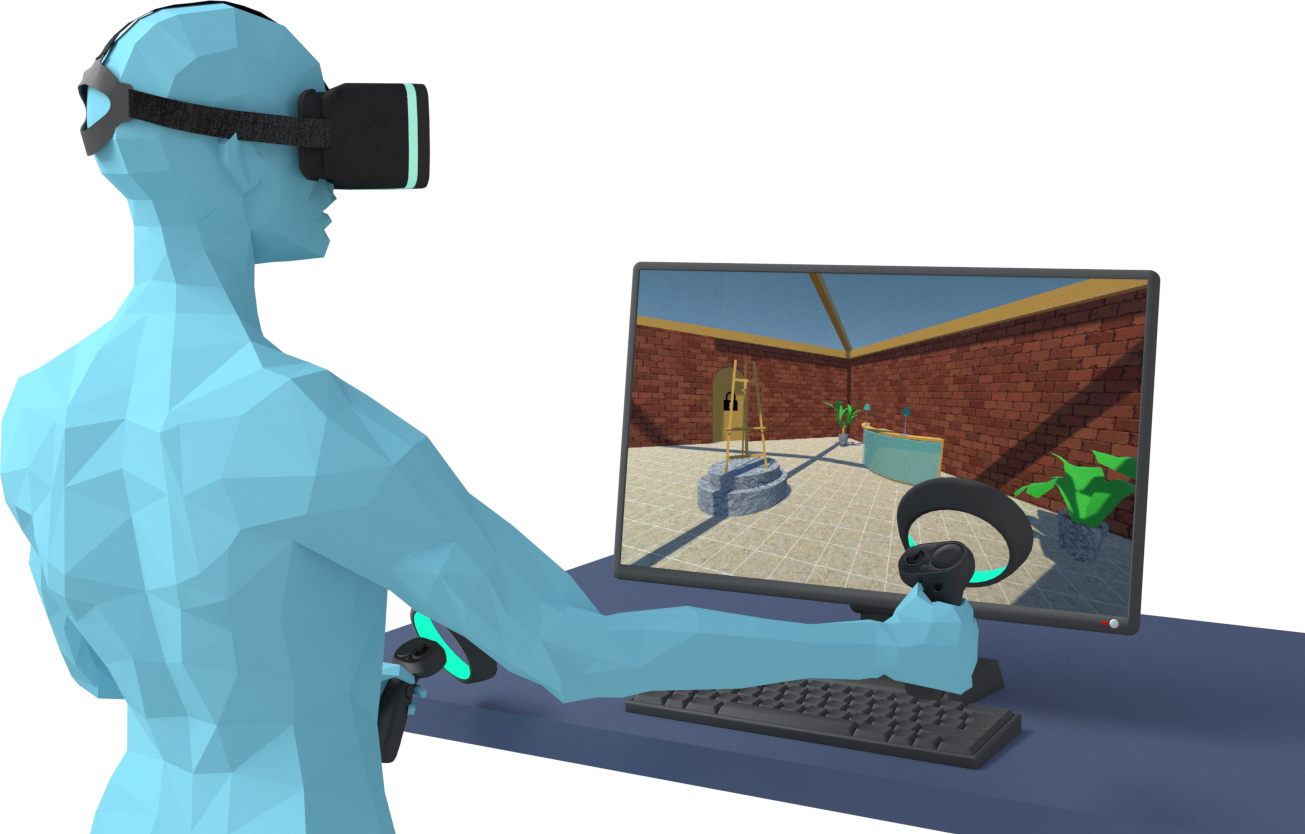
\includegraphics[width=1\textwidth]{imagenes/1/entorno-diffuse-2.png}
\caption{Diagrama de entorno de \MineRVa}
\label{fig:entorno}
\end{center}
\end{figure}

\section{Objetivos}

\subsection{Objetivo principal}

El objetivo de \MineRVa es crear una experiencia inmersiva y en la que el jugador se sienta gratificado al ir resolviendo los pequeños acertijos que se le proponen. Con ello se pretende alcanzar dos objetivos diferentes; por un lado, se busca conseguir que nativos digitales que no suelan visitar museos encuentren en \MineRVa una excusa para hacerlo de manera divertida, y por el otro que usuarios más mayores a los que les gusta visitarlos encuentre en la temática de este proyecto una excusa para jugarlo y disfrutarlo de la misma forma. En cualquiera de los dos casos se espera que, tras completar el juego, la mayoría de usuarios se interesen en visitar museos reales.

Por otro lado, uno de los nichos de jugadores más pequeños y a la vez uno en el que más se ha pensado es en aquellas personas discapacitadas o con movilidad reducida que no pueden físicamente visitar museos. Se espera ayudar especialmente a este colectivo consiguiendo una experiencia equivalente en la medida de lo posible, además de intentar hacerla más amena enmarcándola en el contexto de un videojuego.

\subsection{Objetivos secundarios}

Como objetivos secundarios, se presenta el aprender a desarrollar programas basados en tecnologías de Realidad Virtual, así como a elegir y configurar un entorno adecuado para ello.

Además, al estudiar metodologías de desarrollo de videojuegos reales se espera obtener un mejor conocimiento de cómo funciona un proyecto de desarrollo de estas características.

\section{Estructura del documento}

Este documento ha sido estructurado siguiendo la normativa de \acs{TFM} de la Escuela Técnica Superior de Ingenierías Informática y de Telecomunicación de la Universidad de Granada a través de los siguientes capítulos.

\subsubsection{Capítulo \ref{chap:estado_arte}. \nameref{chap:estado_arte}}

En este capítulo se realiza una presentación del estado actual de las áreas tratadas en este \acs{TFM}, recopilando y exponiendo información relevante relacionada con la Realidad Virtual o el Desarrollo de Videojuegos, entre otras áreas.

\subsubsection{Capítulo \ref{chap:analisis_problema}. \nameref{chap:analisis_problema}}

En este capítulo se introduce este proyecto y se hablará del concepto inicial y la narrativa de \textit{MineRVa}.

\subsubsection{Capítulo \ref{chap:tecnologia}. \nameref{chap:tecnologia}}

Este capítulo recoge los recursos tanto hardware como software que se han utilizado para el desarrollo y documentación de este proyecto.

\subsubsection{Capítulo \ref{chap:metodologias}. \nameref{chap:metodologias}}

A lo largo de este capítulo se hablará de las metodologías de desarrollo de videojuegos y se presentarán las metodologías de trabajo y desarrollo seguidas a lo largo de este proyecto.

\subsubsection{Capítulo \ref{chap:plan_entregas}. \nameref{chap:plan_entregas}}

En este capítulo se presenta y detalla el plan de entregas llevado a cabo para poder cumplir con el plazo de tiempo.

\subsubsection{Capítulo \ref{chap:desarrollo}. \nameref{chap:desarrollo}}

A lo largo de esta capítulo se presenta el trabajo realizado en el marco del plan de entregas del proyecto, además de los resultados obtenidos.

\subsubsection{Capítulo \ref{chap:conclusiones}. \nameref{chap:conclusiones}}

En este proyecto se presenta el resultado final del proyecto, las conclusiones extraídas de su desarrollo y se propone una serie de tareas futuras a realizar.